\begin{problem}{Плакат с эмблемой}{стандартный ввод}{стандартный вывод}{1 секунда}{256 мегабайт}

Уйгун и Вася раскрашивают большой плакат с эмблемой кубка школы по мини-футболу. Эмблема представляет собой стилизованное изображение школьного кубка в виде круга, размещенного внутри прямоугольника. Размеры прямоугольника на плакате $w$~см в ширину и $h$~см в высоту, диаметр круга равен $w$~см, точки касания расположены на вертикальных сторонах прямоугольника в $a$ см от нижнего угла. Область в прямоугольнике ниже мяча должна быть выкрашена красной краской, выше -- синей, сам мяч -- золотой. Для покупки красок ребятам нужно рассчитать площади всех трех областей. Помогите им.

\noindent\centerline{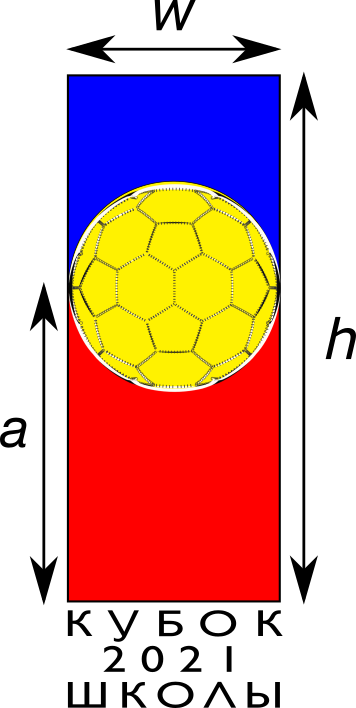
\includegraphics{cup.png}}



\InputFile
В единственной строке заданы три натуральных числа $w$, $h$, $a$ ($1\leq w<h \leq 300$, $\frac{w}{2}\leq a \leq h-\frac{w}{2}$), разделенных пробелами.

\OutputFile
Построчно выведите три вещественных числа~--- площади областей в $\mbox{см}^2$, в порядке снизу вверх: части прямоугольника ниже круга, самого круга, и части прямоугольника выше круга. Точность ответов должна быть не хуже 0.0001.

\Example

\begin{example}
\exmpfile{example.01}{example.01.a}%
\end{example}

\end{problem}

